\FloatBarrier
\chapter{Solution Design}
\label{sec:solution}
\section{Requirements}
\subsection{Context and Goal}

First, we define the context and goal of the solution design. The system is provided as a web-based application, as illustrated in Figure~\ref{fig:sol_context}. The target users include both process modeling experts and domain experts who need to create process models based on documents. To improve modeling efficiency and support non-expert users, the system leverages the LLM service of AutoBPMN.AI for automated model generation. The overall goal is to provide a single, integrated platform in which users can complete the entire modeling process from document upload to model creation, modification and subsequent model management.
\begin{figure}[htb!]
  \centering
  \caption{System context} 
  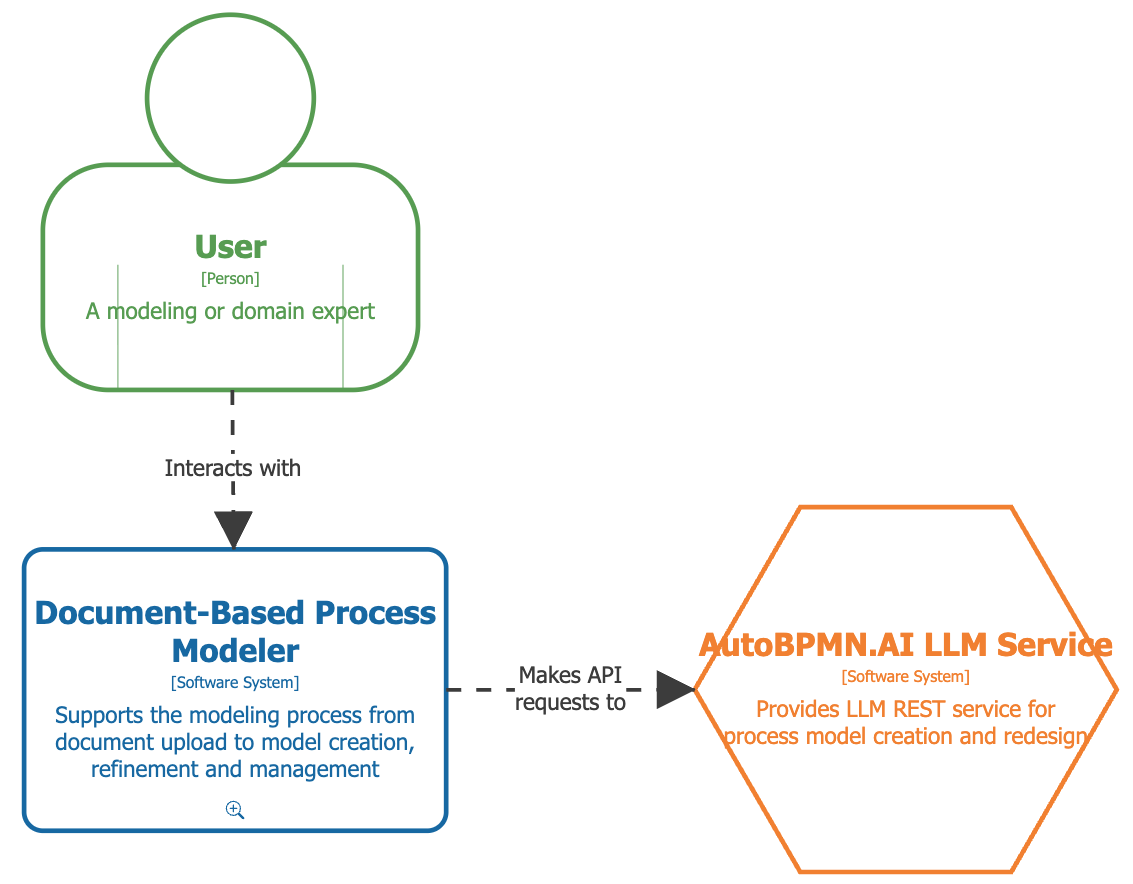
\includegraphics[width=0.8\textwidth]{images/sol_context.png}
  \label{fig:sol_context}
\end{figure}

\section{Requirements Elicitation}
When starting the work the following requirements for the system were defined. 
\label{sec:solution:req}
\begin{figure}[htb!]
  \centering
  \caption{Usage model} 
  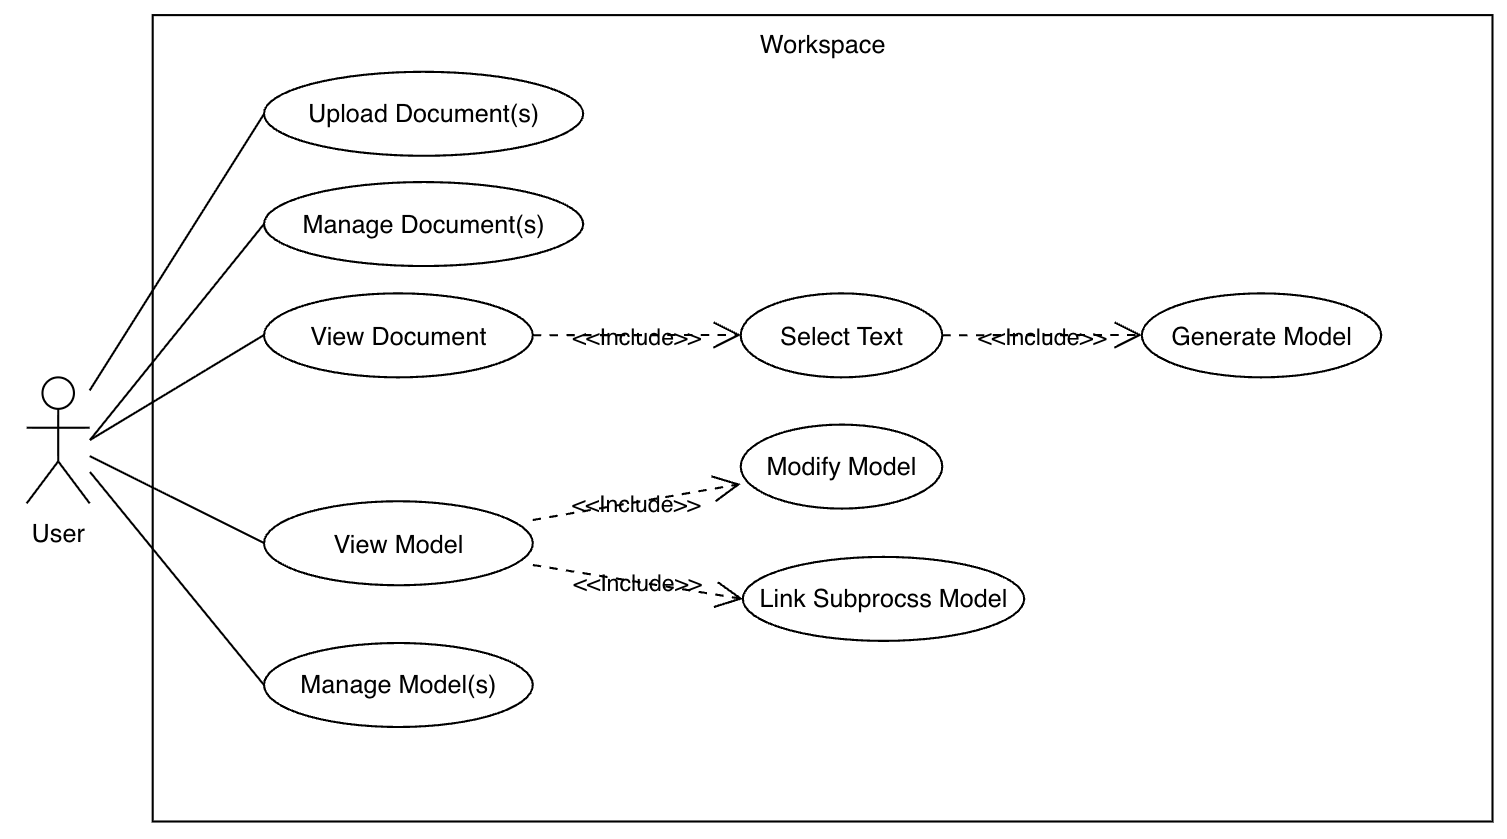
\includegraphics[width=0.8\textwidth]{images/sol_workspace_interaction_usage_model.png}
  \label{fig:workspace_usage_model}
\end{figure}

\section{Requirements Elicitation}
\label{sec:solution:req}



\subsection{Functional Requirements}

Functional requirements define the specific behaviors, actions, and features a system must perform. They outline input/output processing, data manipulation, and user interactions necessary for the system to meet its objectives. These requirements are essential for to build a prototype for this thesis, ensuring system functionality and user needs are met. {LINK TO WIKIPEDA}

It shall allow users to select multiple passages from one document to serve as input for LLM-based process model auto-generation. \\
It shall provide a clear visual link between the text and the generated model.\\
It shall embed the source text within the generated process model for traceability purposes.\\
It shall allow users to establish process-subprocess relationships between models.\\
It shall record user behavior and interactions with the system for analysis purposes.\\
One additional requirement is that the system shall be able to support document update.






\begin{itemize}
    \item \textit{Upload Documents.} The user uploads multiple documents in textual format, e.g., TXT, DOCX, PDF.
    \item \textit{Select Text Passages.} The user selects multiple passages from one uploaded document, then clicks the Generate button to .
    
\end{itemize}


\subsection{Design Constraints}
\begin{itemize}
    \item It shall be implemented as a web-based application.\\
    \item The frontend shall be developed using native web technologies (JavaScript, HTML, and CSS).\\
    \item \textit{Process Model Visualization.} The visualization of the process model shall be implemented using the CPEE Layout\footnote{\url{https://github.com/etm/cpee-layout}} library.\\
    \item \textit{LLM Service Integrati.} The LLM-backed process model generation shall be implemented using the API from AutoBPMN.AI.\\
\end{itemize}

\section{User Interface and Interaction Design}
The desgign overview is described from the user perspective.

Firstly, we define the following concepts to better describe the system:\\
- Project: a use case consisting of one or more documents for which process models needs to be created.\\
- Workspace: the unified page/interface where the modeling workflow is performed, from document upload to model export.\\
- Traceability: the ability to navigate between source text and the corresponding process model.\\
- Project graph: a network-style visualization of relationships among models and documents within a project.\\

The system consists of three main pages: a home page for managing projects, a workspace page where the modeling workflow takes place, and a statistics page for viewing project-related metrics.

\subsection{System Views}
The system is designed to contain three pages: a home page where a user can create a new project or open an existing project, a workspace page where the modeling workflow takes place, and a statistics page where the user can view the statistics of the project.
\subsection{System Views}
The system is designed to contain three pages: a home page where a user can create a new project or open an existing project, a workspace page where the modeling workflow takes place, and a statistics page where the user can view the statistics of the project.
\subsubsection{Workspace}
The layout design of the user interface is shown in the figure~\ref{fig:sol_ui} in a 3-pane layout. The left pane is for document uploading and viewing, the middle pane is for process modeling and the right pane is for process models viewing and project graph visualization. The details are divided as the following: a) Document List b) Document Viewer c) Model Editor  d) Model List e) Project Graph.
\begin{figure}[H]
    \centering
    \caption{Workspace UI Layout} 
    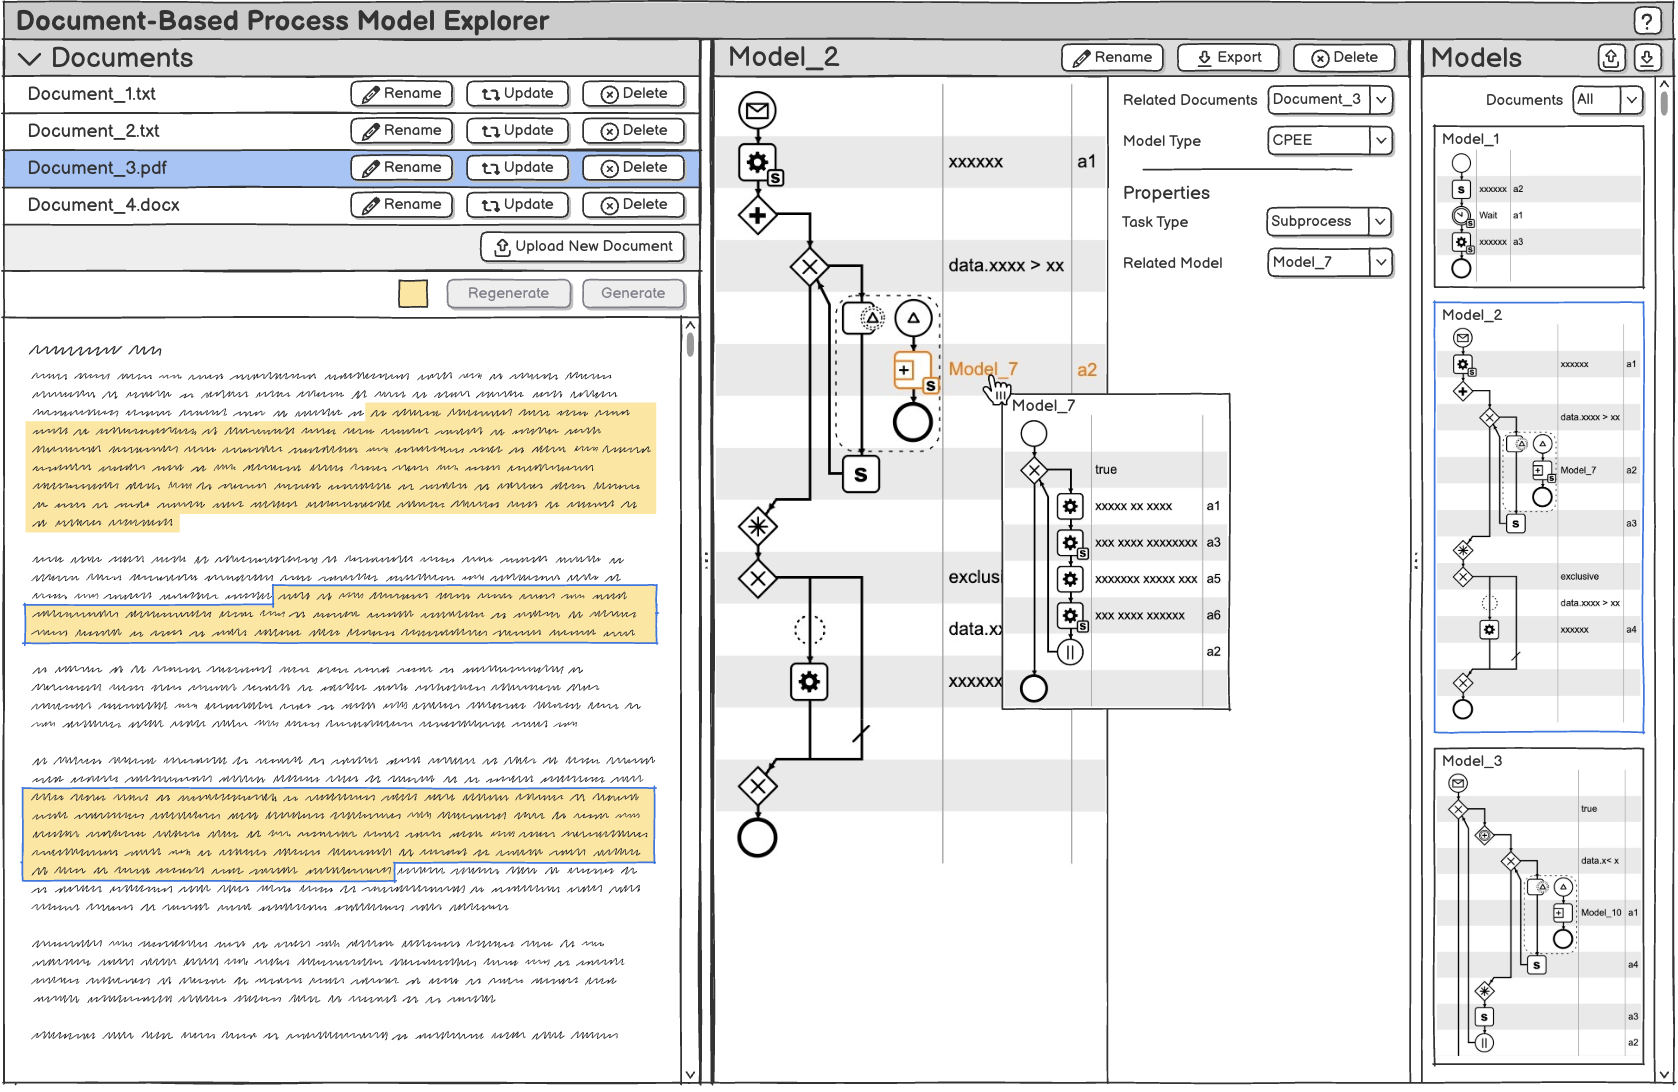
\includegraphics[width=0.8\textwidth]{images/mock-up1.jpg}
    \floatfoot{The user interface layout of the workspace page.}
    \label{fig:sol_ui}
\end{figure}
\section{Modeling Workflow Design}
As the core part of the system, this section describes the modeling workflow that happens in the workspace page in Use Case Diagram.
Figure: .\\
\subsection{Design Difficulities}

\section{Core Functionalities Design}

\subsection{Document Management}
\section{Document Update}
The document update is planned and designed to 
\subsection{Document Interaction}
text selection
text selection editing
\subsection{Process modeling}
\subsubsection{Human-in-the-loop Process Modeling and Version Control}

\subsubsection{Use Case: Model Generation}
By click the button an adavance mode is desgin 
\subsubsection{Use Case: Model Modification}
a. Manual edit
b. Update selected text and apply the changes. 
c. Refinement by sending prompt to LLM:\\
   Input: prompt only and the current Model\\
d. Regeneration:\\
   Input: type a. current model + changed selected text passage b. advanced mode: prompt + current model + changed selected text passage
   
\subsubsection{Use Case: Establishing Process-Subprocess Relationships}

- a review step for each LLM-generated model.
\subsubsection{Augmented Model Data}
\section{Interactive Design Difficulty}




\section{System Architecture}
The system architecture is shown in the figure~\ref{fig:sol_architecture}. The system follows the common web-application client-server pattern. 

\begin{figure}[H]
    \centering
    \caption{System Architecture} 
    
\includegraphics[width=0.8\textwidth]{images/sol_architecture.png}
    \floatfoot{The system architecture of the document-based process modeling tool.}
    \label{fig:sol_architecture}
\end{figure}

\section{Data Model}

\begin{figure}[H]
    \centering
    \caption{The conceptual data model of the system.} 
    
\includegraphics[width=0.9\textwidth]{images/sol_data_model.png}
    \label{fig:sol_data_model}
\end{figure}



